

\documentclass[12pt]{article}

% Language setting
\usepackage[english]{babel}

% Useful packages
\usepackage[margin=1in]{geometry}
\usepackage{amsmath}
\usepackage{graphicx}
\usepackage{pdflscape}
\usepackage{adjustbox}
\usepackage[colorlinks=true, allcolors=blue]{hyperref}
\usepackage{paralist}
\usepackage{cite}
\usepackage{wrapfig}

\begin{document}

% Cover page
\begin{titlepage}
    \centering
    \vspace*{3cm}
    {\LARGE \bf Master Thesis Proposal} \\
    \vspace{1cm}
    {\Large \bf Jonathan Fields} \\
    \vspace{3cm}
    \includegraphics[width=.5\textwidth]{KFSCIS-hrz-COLOR} \\  % Add logo or any relevant image here
    \vspace{3cm}
    \vfill
    {\Large \today}
\end{titlepage}

\newpage

% Table of contents
\tableofcontents
\newpage

\begin{abstract} 
Socially interactive agents (SIAs)  - human-like characters able to have  conversations using verbal and nonverbal communication - have been used in various areas of human--computer interaction. 
Combining SIAs' expressive abilities with the output of large language models (LLMs) enables conversation simulations that directly respond to natural language queries, allowing for more lifelike interactions with less engineering effort (when used without further processing to control their output), when compared to earlier rule-based systems.    
% While machine learning models are increasingly adept at predicting the mood, sentiment, and affect of human users, the ability to simulate expressive communicative and adaptive human behaviors continues presenting a myriad of challenges in allowing such simulations to act as believable "embodiments" of A.I. agents. 
One of the factors influencing SIAs' abilities to retain users' engagement hinges on how the auditory and visual stimuli are coordinated.  Thus, in most cases, the experience of listening to these agents' synthesized speech is improved with visual animations of the 3D character's relevant facial movements synchronized with the spoken utterances. We discuss  current challenges in simulating natural lip synchronization, and propose a system to generate realistic lip, tongue, and jaw movements, as well as ancillary face movements, that can be rendered in real-time for 3D socially interactive agents that can interact with users over the World Wide Web.  We also propose an evaluation methodology for analyzing the lip-synchronization results with a user study.
\end{abstract}

\newpage

\section{Introduction}

%\subsection{Introduction to Embodied Agents}
Socially interactive agents (SIAs)\cite{Gratch2021SIArapport} are interactive systems designed to simulate human-like behaviors, but in virtual space using computer graphics.
%or in-real-life (IRL) physical environments by means of robotic systems. 
Based on the {\em Computers As Social Actors   theory} which states that humans unconsciously apply the same social rules used for human communication to human-computer interaction \cite{Nass1996}, their potential to create more intuitive, engaging, and effective interfaces, such agents have become an increasingly important topic within the field of human-computer interaction (HCI).  The concept of embodied agents extends beyond simple interaction models; these agents can function as fully autonomous cybernetic systems: able to communicate, express emotions, and react adaptively to stimulus, thus simulating aspects of human behavior.  

% \subsubsection{Evolution from ECAs to SIAs}
{Socially Intelligent Agents} represent an evolution from earlier well-known embodied conversational agents (ECAs) \cite{Cassell2000}.  While ECAs were designed to facilitate human-computer interaction by providing a more engaging and intuitive interface than traditional text-based or graphical user interface  systems, they were typically represented as 2-dimensional (2D)  characters capable of basic conversation and task management. However, as AI and machine learning technologies advanced, there was a growing need for agents that could understand and respond to more complex social interactions in 3D virtual environments \cite{Gratch2021SIArapport}.
SIAs are characterized by their autonomy, emotional intelligence, and ability to engage in complex social interactions. Unlike their ECA predecessors, SIAs can detect and respond to users' emotional states, adapt their behavior based on context. These agents are designed to operate in both virtual environments (such as software applications) and physical environments (such as humanoid robots), making them versatile tools for a wide range of applications.
SIAs have been successfully implemented in various fields, demonstrating their potential to enhance user experience. For instance, in customer service, SIAs are used to manage inquiries and resolve issues by understanding the customer's emotional state and responding appropriately \cite{Gratch2021SIArapport}.  These case studies illustrate the significant impact that SIAs can have when effectively integrated into human-computer interaction systems.

% \subsection{Advancements in Emotion Recognition and Empathetic Responses}

% \subsubsection{The Need for Emotionally Intelligent Agents}
% As human-computer interactions become more prevalent in daily life, there is a {\bf growing need for systems that can recognize and respond to users' emotions}. Emotionally intelligent agents are designed to meet this need by incorporating mechanisms for emotion recognition and empathetic response. These agents are particularly valuable in applications where emotional engagement is critical, such as in healthcare, where understanding a patient's emotional state can improve the quality of care \cite{picard1997affective}.

% % \subsubsection{Techniques for Emotion Recognition}
% Emotion recognition in embodied agents is achieved through a combination of techniques, including facial expression analysis, voice tone analysis, and physiological sensors. Facial expression analysis uses computer vision to detect changes in a user's facial features, while voice tone analysis examines the pitch, tone, and rhythm of speech to infer emotional states. Physiological sensors can monitor heart rate, skin conductance, and other indicators to provide additional data on a user's emotional condition.


% \subsection{The Uncanny Valley}
% \subsubsection{Origins and Concept of the Uncanny Valley}
However, as SIAs become more advanced in simulating human-like behaviors, they risk crossing into the {\bf Uncanny Valley}, where slight imperfections in their emotional or nonverbal expressions can lead to discomfort and distrust in users. The concept of the Uncanny Valley was first introduced by Japanese roboticist Masahiro Mori \cite{Mori2012TheValley}. Mori observed that as robots and virtual entities become more human-like, they generally become more appealing to humans. However, when they become almost — but not quite — human-like, they evoke feelings of eeriness and discomfort, a phenomenon he termed the "Uncanny Valley" \cite{Mori2012TheValley}. This concept has become central to discussions surrounding human-robot interaction and, more recently, in the field of virtual agents and deepfake models.

Part of the Uncanny Valley effect, achieving naturalistic facial expressions in virtual agents, also depends on {\bf accurate lip-syncing}, where the phenomenon of coarticulation plays a crucial role in ensuring fluid and realistic speech animations. Coarticulation refers to the phenomenon where the articulation of a phoneme is influenced by preceding or following phonemes, resulting in smooth transitions between sounds. This poses a significant challenge in lip-syncing, as the visual representation of speech needs to account for these transitions, not just isolated phoneme-to-viseme mappings. Traditional approaches that treat phonemes as independent units often lead to unrealistic animations, as they fail to capture the fluidity of natural speech \cite{Edwards2016}.

Recent work has aimed to address this problem by incorporating {\bf coarticulation effects} into lip-sync models. Edwards et al.’s JALI system, for example, separates jaw and lip movements, allowing for more nuanced control over coarticulatory effects, especially in complex speech sequences \cite{Edwards2016}. Similarly, Xu et al. \cite{Xu2013AGames} developed procedural rules to account for the influence of surrounding phonemes, achieving smoother transitions between visemes . These advances enable more realistic speech animations, but they are often tailored for offline animation or pre-rendered content rather than real-time web-based simulations.
One of the most used software for viseme control is Microsoft Cognitive Services TTS, which return viseme codes along with synthesized speech. This approach forces developers to use Microsoft's TTS service for all speech synthesis needs, and does not attempt to remedy the co-articulation problem, nor provide separate lip, jaw and tongue movements, to make the result more realistic.  Futhermore, existing projects have augmented visemes with lip, jaw and tongue movements leading to  more realistic, dynamic simulacra. However, the existing approaches rely on pre-trained models and are designed to be used with animation software packages, instead of web-based simulation.  

 This project {\bf aims to bring realistic, human speech synthesis visualizations in real time to the World Wide Web} by leveraging well-formed observations from previous research existing research such as jaw and lip integration and coarticulation correction.
The goal is to create an algorithm that can take a transcribed text stream and pitch and volume signals from an audio stream and return a stream of viseme codes with activation intensities and durations, combined with additional facial expressions also accompanied by their activation times and durations.  The  output of our algorithm should reflect consideration of how a phoneme's pronunciation may be influenced by preceeding and following sounds (ie. the coarticualtion problem). The output of our algorithm should also reflect consideration of the jaws and lips moving on separate axes to capture various types of speech (ie. whispering, yelling etc). 
%By implementing this algorithm within eEVA, we can have more realistic lip-syncing when compared to Microsoft Cognitive Services' viseme codes.
By combining audio signals from the synthesized speech with phoneme extraction and viseme, our real-time, web-based approach aims to provide a powerful, robust solution for generating dynamic, emotive lip-sync movements on a virtual agent. 

In the following, we provide background information related to the human face and speech in Section \ref{sec:background}, related research on lip synchronization in Section \ref{sec:relatedResearch}, our proposed approach to creating realistic lip synchronization in Section \ref{sec:approach}, and our proposed evaluation approach of  lip synchronization in Section \ref{sec:eval}.
\newpage
\section{Background}
\label{sec:background}

\subsection{Facial Action Coding System (FACS)}
\label{sec:FACS}

The Facial Action Coding System (FACS) \cite{Ekman1976MeasuringMovement} is a widely
used facial coding system for measuring all visible human facial 
movements in terms of the smallest possible muscle Action
Units (AU) causing movement. 

\begin{wrapfigure}[19]{r}{.4\textwidth}
    \centering
    \vspace{-5mm}
    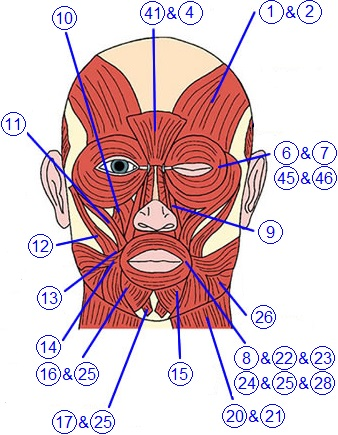
\includegraphics[width=\linewidth]{FaceMuscles-AUs.jpg}
    \caption{Sample AUs of the FACS}
    \label{fig:facs}
\end{wrapfigure}

As shown in Figure \ref{fig:facs}, AUs
are grouped based on their location on the face and the
type of facial action involved. The “upper-face” AUs include
the eyebrows, forehead, and eyelids muscles, e.g., the inner
brow raiser muscle corresponds to AU1; the “lower-face”
AUs include muscles around the mouth and lips; and the
“head and eye movement” AUs include the neck muscles
which move the head, whereas the eye muscles move the
gaze direction.

AUs act as multi-level “switches”, which can create
custom expressions depending on which AUs are acti-
vated/deactivated at a given time. Since not all expressions
require the farthest reach of a muscle, intensity levels are
used to discuss subtle (i.e., less intense) facial movements.
Intensities are annotated from “0” to “E”, with “0” for a
neutral face without any activated AUs, “A” for the weakest
trace of an AU, and “E” for the maximum intensity.
The muscle groups underlying all facial movements
form 44 AUs for facial expressions and 12 AUs for head
and gaze directions.  

As discussed in the next Sections, FACS has been used to create physiologically realistic facial animations for 3D SIA character models.


\subsection{VISAGE Laboratory Socially Interactive Agents}

The verbal and nonverbal communication skills  of  socially interactive agents and their potential at expressing some level of empathy make them effective in scenarios where traditional interventions might fall short \cite{Lisetti2013}.  
The VISAGE lab developed multiple prototypes of socially interactive agents used as the main interface of digital health interventions, showing that users were  31\% more likely to use a web-based health intervention when it is delivered by an SIA compared to with a text-only user interface \cite{Lisetti2013}, and that users are significantly more engaged when the SIA allows speakers to speak freely \cite{LisettiNowExperience}.\cite{Yasavur2014}. 

\subsubsection{empathic Embodied Virtual Agent (eEVA) Framework}
The VISAGE lab has developed the empathetic Embodied Virtual Agents (eEVA) system as 
 a comprehensive virtual agent multimodal framework designed for designing real-time user interactions with agents over the Internet. This framework includes the use of empathetic Embodied Virtual Agents (eEVA) that can engage users in meaningful dialogue using verbal communication (text and speech), and nonverbal communication (facial expressions, body gestures).  It is further implemented so that users can interact with the agents over the Internet, without requiring any installation to increase the SIA's usability and wide access for the population  \cite{PolceanuTimeCONCEPTS}.  The framework was tested with the implementation and delivery of a fully implemented evidence-based digital behavior change health intervention about alcohol uses disorder, which revealed high usability and high acceptance of the agents by users \cite{Amini2021a}\cite{Amini2015}.

\subsubsection{FACSlib}
\label{sec:facslib}

One of the special features of the eEVA framework is its collection of 25 highly expressive 3-dimensional diverse character models.  The 3D model facial animation library - facslib - was custom-made to specifically address the  main limitations of the many existing 3D models used by the SIA community: namely the models do not provide for facial animations corresponding to the FACS system (see Section \ref{sec:FACS}).

Following a similar method as for the development of HapFACS, an open source  software that enables the control of AU-based animations for animating SIAs \cite{Amini2015}, the VisFACS software was created to enabling the visualization of the 3D characters' facial animations at the level of FACS-based Action Units. 
VisFACS built upon the foundation laid by HapFACS, introducing a slider UI and was built in the Vue front-end web framework. For interoperability, the VisFacs app operates as a standalone Mac, PC, and Linux app.

\subsection{GPT Super}

The integration of Generative Pre-trained Transformers (GPT) into the eEVA virtual agent framework marked a significant leap forward in the capabilities of these systems. The evolution to GPT Super introduced advanced natural language processing capabilities, enabling virtual agents to engage in free-speech conversations with users.  Pasternark et al. \cite{Pasternak2024} conducted a study demonstrating the application of a 3D multimodal socially interactive agent (SIA) integrated with the Toyota Human Support Robot (HSR). This integration involved utilizing ChatGPT, a GPT-based large language model, to perform active listening during human-robot interactions (HRI). The study showed that the use of GPT Super allowed this virtual agent embedded within a physical robot (the HSR) to detect and express both verbal and non-verbal cues effectively, thereby enhancing user experience and improving rapport-building during interactions. The synthesis of verbal and non-verbal behaviors facilitated more natural and empathetic communication between the robot and human users.

The incorporation of GPT Super into the virtual agent framework enabled the development of a socially intelligent robot capable of autonomous, human-like responses. This advancement in HRI demonstrates the potential of GPT Super in creating adaptive virtual agents that can engage users in free-text or free-speech conversations.  

\section{Related Research}
\label{sec:relatedResearch}

 The proposed project focuses on synthesizing the visual aspects of speech, specifically how facial animations can accurately reflect spoken language. 
 
 \subsection{Phonemes} 
 \label{sec:phonemes}
 Integral to this endeavor is phonetics, the branch of linguistics concerned with how the human anatomy generates sound and how these sounds are perceived. In linguistics, \textbf{morphemes} and \textbf{phonemes} are the fundamental units of human speech—a \textbf{morpheme} is the smallest unit of language that carries meaning or semantic value, such as a word or a prefix. In contrast, a \textbf{phoneme} is the smallest unit of sound that can distinguish between words in a language, though it may not carry any inherent meaning on its own \cite{Payack2008AWorld}.

\subsection{Viseme to Phoneme Mapping Techniques}

% \begin{figure}[h]
% \centering
% 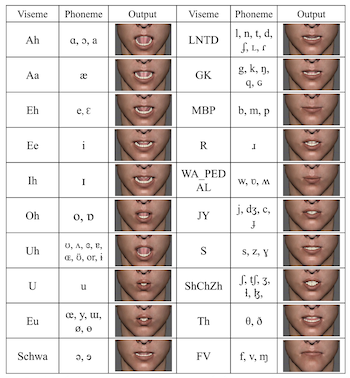
\includegraphics[width=0.8\textwidth]{visemenet.png}
% \caption{List of visemes along with groups of phonemes (in International Phonetic Alphabet format) and corresponding lower face rig outputs that the VisemeNet architecture produces}\cite{Zhou2018visemenet}.
% \label{fig:viseme-mapping}
% \end{figure}

\begin{wrapfigure}[20]{r}{.45\textwidth}
\centering
\vspace{-5mm}
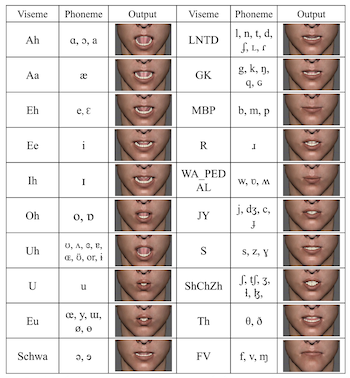
\includegraphics[width=\linewidth]{visemenet.png}
\caption{Visemes, phonemes, and lower face rig outputs \cite{Zhou2018visemenet}.}
\label{fig:viseme-mapping}
\end{wrapfigure}
\subsubsection{Viseme to Phoneme Mapping Techniques}

A viseme (pronounced “vye-seem” and a portmanteau of “visual” and “phoneme”) represents the distinct facial expressions and mouth shapes associated with specific speech sounds or phonemes. One of the pioneering figures in mapping these sounds to their visual counterparts on human faces was \textbf{Cletus Fisher}, whose 1968 research provided a foundational understanding of how consonant sounds are visually perceived and categorized \cite{Fisher1968ConfusionsConsonants.}. Fisher’s work emphasized the classification of consonants into viseme categories based on homophenous consonant confusions observed under controlled conditions, forming \textbf{five viseme categories} based on consonants that were visually indistinguishable when lip-read.

Building on Fisher’s foundation, \textbf{Binnie, Montgomery, and Jackson (1976)} further refined viseme categorization by developing a lipreading screening test that grouped consonants into \textbf{nine homophenous categories} based on place of articulation. Using a set of 20 consonant-vowel syllables, they analyzed the confusion patterns of both normal-hearing and hearing-impaired subjects. The results revealed nine consistent viseme clusters with an overall correct response rate of 79.8\% under ideal viewing conditions \cite{Binnie1976VisualRehabilitation}. Their findings reinforced the idea that place-of-articulation cues are critical for visual speech recognition, aligning with earlier research by \textbf{Woodward and Barber (1960)} \cite{WOODWARD1960PhonemeLipreading}.

\textbf{Massaro (1998)} contributed significantly with his \textit{Fuzzy Logical Model of Perception (FLMP)}, focusing on how auditory and visual cues are integrated during speech perception. Massaro's model has influenced research in the field by demonstrating the importance of combining multiple sources of information—visual and auditory—to create realistic speech animations. His work, which includes the development of the virtual talking face \textit{Baldi}, remains influential in the study of visual speech synthesis and lip-syncing \cite{Massaro1998PerceivingPrinciple}.

Building on these foundations, \textbf{Cappelletta and Harte (2012)} proposed a refined phoneme-to-viseme mapping approach that increased the number of viseme categories to \textbf{20}. Their work focused on improving automatic lipreading systems by capturing subtle visual differences for improved speech recognition accuracy \cite{Cappelletta2012Phoneme-to-visemeRecognition}. \textbf{Xu et al. (2013)} also explored advanced viseme categorization techniques, emphasizing the need for more detailed mappings to account for subtle phonetic distinctions in visual speech \cite{Xu213}.

\textbf{Taylor et al. (2012)} introduced a novel approach by redefining visemes as \textbf{dynamic units of visual speech}. Instead of relying on static mouth shapes representing phonemes, Taylor’s dynamic visemes accounted for the movement of speech articulators, such as the lips and jaw, over time. This model naturally incorporated coarticulation effects—where adjacent sounds influence the current viseme’s articulation—and addressed the asynchrony between visual and acoustic speech signals. By analyzing a corpus of real speech data, the study demonstrated that dynamic visemes better represent the complexity of visual speech, leading to more accurate and visually pleasing speech animations \cite{Taylor2012DynamicSpeech}. Subjective evaluations in the study confirmed that animations generated with dynamic visemes were consistently preferred over those using static viseme models.

In our study, we will adopt \textbf{Microsoft TTS-generated visemes} as the baseline metric for evaluating facial animation and speech synchronization. By using Microsoft’s advanced TTS framework, which integrates well-established phoneme-to-viseme mappings, we ensure consistency and compatibility with widely adopted standards in the field. Given the viseme category expansions suggested in the work of \textbf{Xu et al.} and \textbf{Cappelletta and Harte}, we have chosen to implement \textbf{20 visemes} in our system. This balance allows us to capture subtle phonetic distinctions while maintaining practical utility for real-time applications, ensuring improvements in both visual speech recognition and facial animation fidelity.
\subsection{Viseme Mapping in Digital Animation Production}
\label{sec:useinprod}
In offline animation production and real-time applications like embodied agents, viseme mapping techniques are pivotal in achieving synchronized lip movements. These codes, along with their corresponding durations, ensure that animations accurately reflect spoken language, making production processes more efficient and enhancing the realism of virtual characters \cite{Osipa2010StopRight}. Jan Krejsa (2021) specifically cited practical applications in this area, referencing the influential *Stop Staring* book by Jason Osipa, which provides a detailed guide for animators on creating believable facial animations by hand. Osipa's work is widely regarded as a foundational text in the field of facial animation and lip-syncing, offering techniques that are still relevant today for both traditional and procedural methods \cite{Krejsa2019, Krejsa2021}.

\subsection{Microsoft's Viseme Codes in TTS Systems}
\label{sec:mstts}
Visemes became integral to text-to-speech technology (TTS), where Microsoft’s Speech SDK, for instance, employs a set of 21 viseme codes—a standard reflecting decades of refinement and practical application \cite{GetLearn}. Microsoft's TTS system utilizes an artificial neural network (ANN)-based approach to generate viseme codes and durations. This process, known as forced alignment, ensures that each viseme aligns accurately with its corresponding phoneme in the speech signal \cite{Xu213}. However, while Microsoft’s viseme codes effectively capture mouth shapes, they do not account for other crucial facial movements, such as brow and forehead actions, which are essential for conveying emotion and emphasis in speech \cite{Massaro1998PerceivingPrinciple, Massaro2000ReviewPrinciple}.

In our study, we will adopt Microsoft Cognitive Services' 21 visemes  as the baseline metric for evaluating facial animation and speech synchronization. By using Microsoft’s advanced text-to-speech (TTS) framework, which already integrates well-established phoneme-to-viseme mapping, we ensure consistency and compatibility with widely adopted standards in the field. Moreover, given the viseme category expansions suggested in the work of \cite{Xu213} and \cite{cappelletta2012} , we chose to implement 20 visemes (plus a neutral lip position) in our system. This allows us to strike a balance between capturing subtle phonetic distinctions and maintaining the practical utility needed for real-time applications, ensuring that our system improves both visual speech recognition and facial animation fidelity over Microsft's current offering.

\subsection{Data-Driven Approaches}
Data-driven approaches have gained prominence due to their ability to learn from large datasets and produce highly realistic animations. These methods,   including models like JALI, VisemeNet, and FaceFormer which we discuss next, 
leverage machine learning techniques to automatically map phonemes to visemes and generate corresponding facial animations.

{\bf JALI (Jaw and Lip Integration)} model  \cite{Edwards2016}  represents a significant advancement in the generation of realistic lip-sync animations, particularly in addressing the challenges of coarticulation.

\begin{wrapfigure}[20]{r}{.5\textwidth}
\centering
%\vspace{-mm}
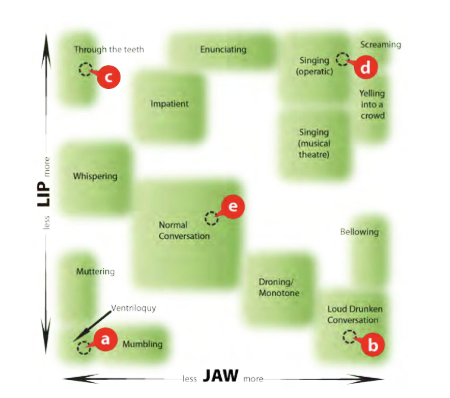
\includegraphics[width=\linewidth]{jali.png}
\caption{Speaking styles captured by the JALI viseme field \cite{Edwards2016}.}
\label{fig:jali-viseme-field}
\end{wrapfigure}

The JALI  model integrates procedural and data-driven approaches to generate expressive lip-synchronized facial animations. This system is built upon the popular FACS (Facial Action Coding System) framework \cite{F} discussed in Section \ref{sec:relatedResearch}, and its unique feature is the separation of jaw and lip movements, which allows for a more nuanced representation of speech. The JALI workflow takes a speech transcript and audio signal as inputs, and through a combination of forced alignment and audio signal analysis, it generates both viseme codes and action units that are procedurally modulated to animate a 3D character's face.

JALI’s procedural components include the precise control over the jaw and lip on seperate axes, which are modulated based on the audio features like volume, pitch, and formants--those frequency regions of relatively great intensity within a given sound spectrum. Plotting these jaw and lip movement intensities along an x and y axis yields regions consistent with various styles of speech like whispering or yelling. For example, the minimum activation of both jaw and lips would yield a style of speech consistent with ventriloquism, adding slightly more lip activation would yield mumbling wheras slightly more jaw activation would yield murmuring (see Figure \ref{fig:jali-viseme-field}). This approach ensures that the resulting animations are both expressive and realistic, closely matching the performance of professional animators and performance capture systems. The JALI system is designed to be integrative, allowing further artistic refinement, and is particularly useful in environments where performance capture might be impractical or where detailed animator control is desired.

\textbf{VisemeNet (2018)} \cite{Zhou2018visemenet} is another data-driven approach, utilizing a Long Short-Term Memory (LSTM) neural network-based model to generate realistic lip-sync animations. The model was trained on several well-known datasets, including BIWI, SAVEE, GRID, TCD-TIMIT, and CREMA-D, to predict viseme sequences from audio inputs. VisemeNet’s architecture also incorporates LSTM layers, which captures temporal dependencies in sequential data. The network architecture is designed to handle complex speech patterns by segmenting the audio into phonetic groups, which are then mapped to corresponding visemes. 

\label{ref:faceformer} \textbf{FaceFormer (2022)} \cite{Fan2022} introduces a Transformer-based autoregressive model for speech-driven 3D facial animation. Unlike earlier methods that rely on short audio windows, FaceFormer encodes long-term audio context, enabling it to generate temporally stable and highly realistic facial animations. The model integrates self-supervised pre-trained speech representations, which helps mitigate data scarcity issues. Additionally, FaceFormer incorporates two biased attention mechanisms—cross-modal multi-head attention for aligning audio and motion modalities and causal multi-head self-attention with periodic positional encoding for improved generalization to longer audio sequences. FaceFormer has demonstrated superior performance compared to state-of-the-art methods, particularly in lip-sync accuracy and overall realism of the 3D character.

\subsection{LipNet for Automated Lipreading}
\label{ref:lipnet}
LipNet is one of the first end-to-end sentence-level lipreading models, developed by \cite{AssaelLIPNET:LIPREADING}. Unlike earlier systems that focused solely on word classification, LipNet predicts entire sentences from sequences of video frames. The system leverages spatiotemporal convolutions, recurrent neural networks (RNNs), and the connectionist temporal classification (CTC) loss to perform accurate sentence-level sequence prediction.

In a benchmark evaluation on the GRID dataset, LipNet demonstrated a 95.2\% sentence-level word accuracy, outperforming both human lipreaders and previous state-of-the-art models by a significant margin. This model is particularly relevant to our project’s quantitative evaluation as it showcases the potential of deep learning architectures in decoding continuous lip movements. LipNet's application of spatiotemporal convolutional neural networks (STCNNs) combined with a bidirectional GRU enables it to capture both spatial and temporal dynamics of facial motion, making it an excellent candidate for evaluating algorithms that aim to improve lip synchronization.

Additionally, LipNet's success highlights the importance of sentence-level predictions rather than isolated word-level predictions, which aligns with the goals of our study. By incorporating LipNet's framework or findings, we aim to strengthen the quantitative evaluation section of our work (see Section \ref{sec:eval}), providing a comprehensive assessment of lip synchronization algorithms in natural communication contexts.

\cite{AssaelLIPNET:LIPREADING} further emphasizes the system's ability to generalize across previously unseen speakers (never used in the training set), reporting an 88.6\% accuracy on such data. This ability to generalize beyond the training dataset is critical for real-world applications of lip synchronization and will serve as an important baseline in our quantitative analysis.


\section{Proposed Approach}
\label{sec:approach}

\subsection{New Platform Enhancements with React and ECMAScript 6}

To facilitate the eEVA framework maintenance  and to take advantage of modern JS language features that would make modifying and running the application much simpler, we propose planned improvements below. 

\subsubsection{ECMAScript 6 (ES6)}

Transitioning to the more modern ECMAScript 6 (ES6) -- the latest of a set open source standards for surrounding the Javascript programming language, formalized by the European Computer Manufacturers' Association\cite{ECMA-262International} -- allows for the removal of Anuglar1 dependency injection in favor of language-native import statements\cite{ECMA-262International}\cite{JavaScriptMDN}\cite{ExploringES6}. This also means that the Bower front-end package manager, which had been deprecated since 2015, could be replaced by Node Package Manager (NPM). Additionally, the introduction of the React.js frontend web framework allows easy adding of User Interface (UI) elements and manages state using the reactive programming paradigm. This reactive programming paradigm can  furthermore be extended from simple UI, to also encapsulate the nuances of conversation-based interaction with a virtual agent.

\textbf{Import Statements and Classes}: ES6 introduced modules and classes, which allowed developers to structure code more effectively. In particular, import statements and classes in ES6 can replace older patterns like Angular’s dependency injection and Bower for package management. This transition to ES6 simplifies the codebase, making it more modular and easier to maintain.

\textbf{Replacing Angular Dependency Injection}: ES6 modules provide a native way to import and manage dependencies, reducing the need for Angular’s dependency injection system. This shift allows for more flexibility and reduces the complexity of the application architecture.

\textbf{Replacing Bower}: With the advent of ES6 modules, package management became more streamlined, reducing the reliance on tools like Bower. This transition not only modernized the development process but also aligned it with current best practices in web development.

The adoption of ECMAScript 6 will be  crucial in modernizing the implementation of Dr. Lisetti’s virtual agent frameworks, ensuring that the code is both future-proof and maintainable.

\subsection{Building Web-Based Interfaces with React.js and Chakra UI}

To facilitate user interaction and data collection, {\em React.js} alongside the {\em Chakra User Interface} component library will be used to build web-based interfaces. As discussed below, this setup is ideal for rapidly developing user interfaces that are both intuitive and highly customizable, which will be critical for the lip-reader studies (see Figure \ref{fig:chakra}).

\begin{wrapfigure}[23]{r}{.5\textwidth}
    \centering
    \vspace{-3mm}
    \includegraphics[width=\linewidth]{chakra.png}
    \caption{eEVA's webbased UI (Chakra and React.js) controlling visemes lip-shapes on the Amy character. }
    \label{fig:chakra}
\end{wrapfigure}
\subsubsection{Reactive programming and conversational agents} 

\textit{React.js}: React.js is a front-end web framework, developed at Meta, provides a reactive, stateful base from which the cybernetic functioning of the agent, as well as UI controls can be easily implemented.
While {\em React} works by managing state with transitional state machines (TSM), this same reactive programming approach can be extended to encapsulate the nuances of a conversation with a socially interactive agent. 

For example, we can use custom, domain-specific states like "talking," or "listening" and so on. This approach allows the agent to respond adaptively to a given change in the dynamic of the interaction, opposed to relying on lower-level asynchronous handling mechanisms like callback functions or promises--thus allowing more complexity surrounding the agents' responses under a myriad of possible combinations of conditions.

\subsubsection{Chakra User Interface}

{\em Chakra UI}  is a component library that works with React that provides many useful common UI components such as sliders, switches, and menus.

 The interface design and functionality will be supported by Chakra UI, which offers a wide range of pre-built, accessible components that can be tailored to fit the specific needs of the user studies. The interface will allow users to interact with the virtual agent, observe the lip-syncing in action, and provide real-time feedback on the accuracy and realism of the animations.

During our evaluation stage (discussed in Section \ref{sec:eval}), data collection and analysis will be managed by React.js, which will handle the dynamic rendering of the interface and the gathering of feedback from users. The data gathered through this interface will be crucial for refining the virtual agent’s behavior and improving the system’s overall performance. 

Real-time interaction with the virtual agent will be supported by the web-based interface, enabling participants to see immediate changes in the lip-syncing as they interact with the system. This real-time feedback loop will be essential for ensuring that the system can be fine-tuned effectively based on user input.

Such technical improvements will furthermore enable an easier of the integration of our novel text-to-phoneme and phoneme-to-viseme modules, which we discuss next.

\subsection{Text-to-Phoneme and Phoneme-to-Viseme Mapping}
Our approach to text-to-phoneme and phoneme-to-viseme mapping builds on techniques discussed in previous research, such as the mappings introduced by \cite{Xu2013AGames}  Microsoft’s Neural TTS system. In a similar manner to Xu’s 21-viseme system, we aim to achieve efficient real-time performance by simplifying the phoneme set and mapping them to a corresponding set of visemes. This process begins with analyzing synthesized speech text to identify phonemes, which are the smallest sound units of speech (see Section \ref{sec:phonemes}). These phonemes are then mapped to their corresponding visemes, which visually represent those sounds on the virtual agent's face.

However, where we will diverge from the approach by \cite{Xu2013AGames} is in how we address certain limitations in phoneme identification. Our system will employ the \textit{Double Metaphone algorithm} during the text-to-phoneme conversion phase to improve accuracy, particularly for handling variations in pronunciation and accents. This phonetic algorithm developed by \cite{PhillipsScholar} encodes words into phonetic codes approximating their pronunciation, allowing for more reliable phoneme identification, even when the pronunciation differs from standard forms.

While the basic phoneme-to-viseme mapping provides a strong baseline, our approach introduces additional refinements to handle variations in speech delivery such as tone, speed, and emphasis. These are crucial for improving the fidelity of the lip-sync across different contexts and ensuring that the visual speech output remains realistic, even in dynamic or fast-paced conversations.

In our system, FACS AUs (see Section \ref{sec:FACS}) will be used to improve the realism of the speech production movements. While the primary focus will be on generating accurate lip shapes using viseme codes, we will use Paul Eckman's Facial Action Coding System's (FACS) action units (AUs)\cite{Ekman1978} to augment these lip shapes with realistic jaw and tongue movements. This augmentation ensures that speech-related movements appear more fluid and natural without introducing emotional expressions, which are reserved for future studies.

\subsection{Basic Logic for Viseme Duration Estimation}
Once phonemes are mapped to visemes, the next step involves estimating the duration of each viseme. Drawing from earlier studies, such as \cite{cappelletta2012}, which used phoneme properties for mapping, we apply basic rules for determining viseme durations based on the characteristics of each phoneme and its context. For example, vowels typically require longer viseme durations due to their sustained sound, while consonants often need shorter, more abrupt movements. This ensures fluidity in the virtual agent’s lip-sync.

\subsection{Audio Signal Extraction for Fine-Tuning}
To refine viseme durations and introduce more nuanced facial movements, we extract audio signals from the synthesized speech. This approach is informed by  \cite{Taylor2012DynamicSpeech}, which highlighted the importance of incorporating co-articulation effects and dynamic audio cues. By analyzing the pitch, rhythm, and intensity of the audio, our system adjusts viseme timing and intensity. For instance, if a phoneme is emphasized in the speech, the corresponding viseme's duration and intensity will be adjusted to reflect that emphasis, creating more expressive and synchronized lip movements. This differentiation between lip movements (which are phoneme-dependent) and jaw movements (which correlate with pitch and volume) enhances the system’s overall realism.

This multi-layered approach ensures the system can maintain low latency while integrating complex audio-visual interactions, crucial for real-time applications like virtual agents or AI-driven conversations.  The absence of model training ensures that our operations remain lightweight and fast. Unlike previous designs that required significant computational resources for real-time processing, our proposed system aims at being optimized for immediate interaction, enabling smooth real-time execution within web environments.
\section{Proposed Evaluation}
\label{sec:eval}
Our evaluation strategy draws on the insights from related work in speech-driven animation and human facial expression modeling. We will conduct both quantitative and qualitative evaluations. Indeed, as noted in \cite{Fan2022}, ``[g]iven the many-to-many mappings between upper face motions and the speech utterance, it is suggested that qualitative evaluations and user studies are more proper for evaluating the quality of speech-driven facial animation than using quantitative metrics'' (see Section \ref{ref:faceformer}). This observation underscores the need for subjective assessments when evaluating the nuances of lip synchronization, as purely quantitative metrics may fail to capture the full range of user experience and animation quality.

\subsection{Quantitative Evaluation}

To quantitatively evaluate the accuracy of our lip-synchronization algorithm, we perform two key comparisons: first, a direct comparison of our model’s output using the state-of-the-art LipNet model \cite{AssaelLIPNET:LIPREADING}, and second, a comparison of our model’s generated visemes with those produced by Microsoft Cognitive Services.

For the first comparison, we leverage the LipNet framework, which achieves a 95.2\% sentence-level word accuracy on the GRID corpus. LipNet is capable of mapping video sequences of lip movements to corresponding transcriptions of spoken sentences by utilizing an artificial neural network (ANN). This model serves as an effective benchmark for assessing how well our algorithm replicates lip movements in sync with the corresponding text. Our algorithm’s output will be directly compared to LipNet’s predicted transcriptions on a set of lip-synced video sequences of the virtual character. Accuracy is computed by analyzing word error rates (WER) and character error rates (CER) between the transcriptions generated by our lip-synced videos and LipNet’s predictions, similar to the evaluation metric used in \cite{AssaelLIPNET:LIPREADING}.  We will have our system output videos which can then be used as inputs into the pretrained LipNet model.

Additionally, the use of word error rate (WER) and character error rate (CER) as evaluation metrics is standard in speech recognition and visual speech perception \cite{KlakowTestingQ}. These metrics account for the differences between predicted and ground-truth sequences, including insertions, deletions, and substitutions, and are calculated as follows:

\[
WER = \frac{S + D + I}{N}
\]
\[
CER = \frac{S + D + I}{C}
\]

where $S$, $D$, and $I$ represent substitutions, deletions, and insertions, respectively, and $N$ and $C$ represent the total number of words or characters in the reference.

In addition to LipNet, we will compare our system’s output with that of Microsoft Cognitive Services’ Viseme API. This API generates viseme sequences based on audio input, providing a phoneme-to-viseme mapping. Our algorithm’s output will be directly compared to the viseme sequences provided by the Cognitive Services API. Evaluation metrics include the alignment of visemes with the corresponding phonemes as well as the temporal accuracy of the transitions between visemes. This evaluation allows us to assess how closely our system’s generated visemes align with expected speech viseme patterns, ensuring a natural and coherent lip-synchronization experience.

The results of these evaluations will be presented through a detailed analysis of WER and CER for the LipNet-based comparison, alongside accuracy metrics derived from viseme alignment and transition timing for the Microsoft Cognitive Services evaluation. By employing these two comparison methods, we ensure a robust and comprehensive evaluation of our lip-synchronization algorithm’s performance in real-world conditions.

\subsubsection{Proposed Analysis for LipNet Evaluation}

For the LipNet evaluation, we will measure lip-sync accuracy using Word Error Rate (WER) and Character Error Rate (CER) \cite{KlakowTestingQ}, which are computed as follows:

\[
WER = \frac{S + D + I}{N}
\]
\[
CER = \frac{S + D + I}{C}
\]

where $S$, $D$, and $I$ represent substitutions, deletions, and insertions, and $N$ and $C$ are the total number of words or characters in the reference sample.

\subsubsection{Proposed Analysis for Microsoft Viseme Codes Evaluation}

For Microsoft’s Viseme Codes, we will not expect an exact match but will focus on improving the realism and user experience. We will assess Viseme Alignment Accuracy (VAA) and Viseme Recognition Rate (VRR) in lip-reading tasks, similar to the approach used by \cite{Santos2023ALipreading}.

\[
VAA = \frac{A_{\text{correct}}}{A_{\text{total}}}
\]
\[
VRR = \frac{v_{\text{correct}}}{v_{\text{total}}}
\]

where $A_{\text{correct}}$ and $v_{\text{correct}}$ represent correct viseme alignments or recognitions, and $A_{\text{total}}$ and $v_{\text{total}}$ are the total number of visemes.

\subsection{Subjective Evaluation}
\subsubsection{Proposed Lip-reader Evaluation}

For the proposed lip-reading evaluation, participants will view animation sequences acted out by a virtual agent through a web-based UI, with the audio removed. The animations will depict sentences presented visually, modeled after CUNY-style sentence tests \cite{Altieri2011SomeL}, and will allow for the assessment of participants’ visual-only speech recognition abilities. Participants will not be provided with any auditory cues, making this a purely visual task aimed at evaluating the accuracy of lip-reading or viseme recognition \cite{Altieri2011SomeL}.

The test will consist of short sentences presented one at a time. After each animation, participants will be prompted to submit their responses, either by typing out the sentence they perceived or by selecting from a multiple-choice set of possible responses. This approach, commonly used in lip-reading evaluations, standardizes responses and facilitates controlled analysis \cite{Altieri2011SomeL}.

We will compute metrics such as **Word Accuracy (WA)**, **Sentence Accuracy (SA)**, and **Viseme Recognition Rate (VRR)** to assess performance. These are defined as follows:

\[
WA = \frac{n_{\text{correct words}}}{n_{\text{total words}}}
\]
\[
SA = \frac{n_{\text{correct sentences}}}{n_{\text{total sentences}}}
\]
\[
VRR = \frac{v_{\text{correct}}}{v_{\text{total}}}
\]

The data will be logged via the web-based UI and analyzed to improve the synchronization of viseme animations with speech content.

\subsubsection{Proposed User Study Evaluation}

% In our user study, we will integrate the Tcha-Tokey et al. (2016) questionnaire \cite{TchaTokey2016}, which evaluates various dimensions of user experience in Immersive Virtual Environments (IVEs). This questionnaire will assess components such as presence, immersion, engagement, flow, usability, and emotional response.

% During the VR session, we will intermittently collect conversational feedback. The feedback will be simple and conversational, such as:

% \begin{itemize}
%     \item "How immersed do you feel right now?"
%     \item "What part of the environment has been the most engaging for you?"
%     \item "How comfortable are you with the controls?"
% \end{itemize}

% This feedback will allow us to capture users’ immediate reactions, complementing the more formal post-session questionnaire.

% After completing the conversation with the agent, participants will fill out the full Tcha-Tokey UX questionnaire. Additionally, we will incorporate open-ended questions to encourage reflection on both positive and negative aspects of the experience. The data gathered will offer both qualitative and quantitative insights into the users’ overall experience, helping us identify areas for potential improvements in usability, engagement, and emotional impact.

% \subsubsection{Proposed Analysis for User Study with VR Questionnaire}

% In the user study, we will assess participants’ experiences using the Tcha-Tokey et al. (2016) questionnaire \cite{TchaTokey2016}. The following metrics will be calculated:

% \textbf{Usability Score (US):} This score will be derived from participants’ responses to the usability-related questions in the questionnaire. Each question is rated on a Likert scale, and the overall score is calculated as:

% \[
% US = \frac{\sum_{i=1}^{n} Q_i}{n}
% \]

% where $Q_i$ is the score for each usability question, and $n$ is the total number of usability-related questions.

% \textbf{Overall Experience (OE):} The overall experience score will reflect participants’ general satisfaction and engagement. This will be calculated as:

% \[
% OE = \frac{\sum_{i=1}^{m} Q_j}{m}
% \]

% where $Q_j$ is the score for each experience-related question, and $m$ is the total number of experience-related questions.

% \textbf{Immersion Index (II):} The immersion index will be calculated based on participants’ ratings of their sense of presence and immersion within the virtual environment. The formula is:

% \[
% II = \frac{\sum_{i=1}^{k} I_i}{k}
% \]

% where $I_i$ is the score for each immersion-related question, and $k$ is the total number of immersion-related questions.

% By combining real-time feedback, Likert-scale questionnaire data, and qualitative insights, we will gain a holistic understanding of user engagement and system usability, providing critical insights for improving our lip-synchronization and user experience.


In this portion of the evaluation, participants will interact with a rule-based conversion engine, designed to yield consistent results (necessary for experiment design), these generated texts will be spoken by the Socially Interactive Agent (SIA). 

This study will focus on evaluating whether the proposed approach can outperform existing solutions like the Microsoft TTS API in generating accurate and natural lip-syncing. The primary goal will be to determine if the system can produce better lip-syncing results than those provided by the Microsoft TTS API, which already generates viseme codes and durations for synthesized speech. 

We will conduct the study with an experimental design.
Participants will be randomly assigned to engage to two conditions: one condition with the SIA using our lipsynch approach, and the other with the SIA using the Microsoft TTS API. Participants will provide feedback on the naturalness, accuracy, and overall user experience of the lip-syncing after their intreaction with the SIA. 

The study will measure key aspects such as perceived naturalness of the lip-syncing, the accuracy of viseme durations, and participant satisfaction. These metrics will help assess whether the proposed system provides a significant improvement over existing solutions.

This user study will be designed to provide direct, practical feedback on the system’s performance, guiding further development and refinement to achieve the best possible outcomes.

\section{Ethical Considerations}

As this system involves the development of a highly realistic virtual agent, ethical considerations must be taken into account. This includes ensuring transparency with users about the system's capabilities and limitations, particularly in sensitive applications such as healthcare or counseling. Additionally, future development will focus on maintaining user trust by providing clear indications of the system's artificial nature.

\bibliographystyle{plain}
\bibliography{references}
\end{document}


